\documentclass[11pt]{amsart}


\usepackage{graphicx}
\usepackage{amsmath}
\usepackage{amssymb,amsthm,bm,url,paralist,tabls,hyperref,amscd}
\usepackage{caption}
\usepackage{subcaption}

\newtheorem{thm}[equation]{Theorem}
\newtheorem{prop}[equation]{Proposition}
\newtheorem{lem}[equation]{Lemma}
\newtheorem{cor}[equation]{Corollary}
\newtheorem{conj}[equation]{Conjecture}
\newtheorem{rem}[equation]{Remark}
\newtheorem{examp}[equation]{Example}
\newtheorem{defn} [equation]{Definition}
\theoremstyle{remark}	  \newtheorem*{remark}{Remark}



\newcommand{\pre}[2][f]{{#1^{-1}\left(#2\right)}} 
\newcommand{\set}[1]{\left\{#1\right\}} 
\def\ZZ{\mathbb Z}
\def\RR{\mathbb R}
\def\QQ{\mathbb Q}

\numberwithin{equation}{section}
\usepackage{varioref}
\labelformat{section}{Section~#1}
\labelformat{subsection}{Section~#1}
\labelformat{subsubsection}{Section~#1}
\labelformat{figure}{Figure~#1}
\labelformat{table}{Table~#1}
\labelformat{defin}{Definition~#1}
\usepackage[letterpaper,margin=1in]{geometry}

\title{Topological Data Analysis: The Geography of Countries}
\author[Andrew Banman]{Andrew Banman \\  Department of Mathematics, Statistics, and Computer Science \\  Macalester College \\   St. Paul, MN 55105}




\date{December 4, 2015}

\begin{document}




\maketitle
\begin{abstract}
\noindent
In this paper I analyze the question of whether or not the countries of the world are evenly divided into first and third world categories using techniques of persistent homology and standard clustering algorithms. Data on health and economics is drawn from the GapMinder project and analyzed alongside geographic data of countries. Preliminary evidence is found in support of the existence of some division between countries of the world.
\end{abstract}


\section{Introduction}

Counties are often dived into two categories: a \emph{1st world}, comprised of developed western-style countries, and a \emph{3rd world} comprised of less-developed countries. The Gapminder project attempts to challenge this distinction by showing the lack of correlation between such indicators as life expectancy and income per person.\cite{gapminder}  The topology of this data can also provide insight into this question, particularly by incorporating the geography of countries alongside social indicators. Persistent homology reveals that there exist at least two connected components in the data, representing distinct groups of countries. These connected components are illuminated by $k$-means clustering algorithm, which provides an interesting comparison with zero-order homology as a clustering algorithm in its own right. This paper begins with a brief overview of homology and persistent homology before applying these techniques to data drawn from the GapMinder project. 

\section{Simplicial Homology}

Generally speaking,  homology is concerned with counting the holes of varying dimensions in topological spaces. Homology groups provide a rough approximation to the homotopy groups that is more intuitive and, as it turns out, easily computed via linear algebra. 

Begin with a simplicial complex $K$, a space with a triangulation, and define the set of $n$-dimensional cycles $Z_n$ in the triangulation. Now, let $B_n$ be the set of all cycles that also represent the boundary of some $(n+1)$-simplex in $K$. Then the homology group is formed by modding the cycles out by the boundaries, leaving just those cycles that are holes. 


\begin{defn}\cite{Crossley}
  The $nth$ \emph{homology group} of a simplicial complex $K$ is the quotient space 
  \[ H_n(K) = \frac{Z_n}{B_n} \]
\end{defn}

It is imporant to  note that there is a rich underlying structure of linear algebra in these definitions. Cycles and boundaries may be thought of as the kernals and images of (linear) boundary maps that connect the spaces of subsets of $n$-simplicies in $K$. Then the problem of finding the the order of each homology group, which is the real quantity of interest, is simple linear algebra. These orders are known as the Betti numbers. 
 
\begin{defn}  The $ith$ \emph{Betti Number} of a simplicial complex $K$ is the order of the $ith$ homology group of $K$, e.g. $b_i(K) = ||H_i(K)||$.  
\end{defn}

For example, $b_0$ counts the number of 0-holes, which can be thought of as the number of connected components. Likewise $b_1$ counts the number of 1-holes, or topological circles, and $b_2$ counts the number of 2-holes, or trapped volumes, in the space.

\section{Persistent Homology}

The definitions above require one to know the topological space before calculating homology groups, but what if instead there is only data that may or may not represent a particular topological space? Given a set of data representing points in Euclidean space, a ``point cloud'', there is a natural simplicial complex construction known as the Czech Complex. It turns out that this construction quickly grows to be too large to be convenient in calculations, but there is a suitable approximation known as the Vietoris-Rips Complex that is less computationally expensive. I refer to (Ghrist) for a technical  explanation of why this is the case. 

\begin{defn} \cite{ghrist}  Given a set of points in Euclidean space, the  \emph{Vietoris-Rips Complex} $R_\epsilon$ is the abstract simplicial complex whose $k$-simplices are determined by unordered ($k$+1)-tuples of points whose closed $\epsilon/2$-ball neighborhoods have a point of common intersection. 
\end{defn}

In other words, a set of $k+1$ points forms a $k$ simplex in $R_e$ only if the intersection of the  neighborhoods around each point is not empty. The size of these neighborhoods is controlled by the parameter $\epsilon$, a characteristic distance often called the ``filtration time'' in this context. Then the question arises what is the optimal filtration time to capture the \emph{true} topology of the data? Of course, the answer is that no such preferred parameter value exists. 


Instead of choosing a particular $\epsilon$, we consider a simplicial complex chain, a series of nested $R_\epsilon$ with increasing filtration time. Then a feature is said to reflect the topology if it \emph{persists} in multiple complexes over a significant range of $\epsilon$. Rather than finding specific Betti numbers, we record the intervals over which elements of the homology groups persist. Barcodes are conventionally used to display these intervals, but a persistence diagram provides a more concise visualization by displaying each order homology in a single chart. Features located near the the diagonal are considered noise, as they vanish almost immediately after coming into existence. Consider the following example of the sphere. 

\begin{examp}
The homology of the sphere is well known, and it provides a  perfect example for our purposes. First, we randomly sample points from the sphere to generate the point cloud. There are a number of software packages with functions to calculate the homology intervals, such as \emph{pHom} for R and \emph{JavaPlex} for MatLab. Observe the 2-hole persisting until about $\epsilon = 1$ and the 0-hole persisting the full duration of the filtration. These agree with the Betti numbers $b_0(S^2) = 1$ and $b_2(S^2) = 1$. Note that every 1-hole vanishes soon after it comes into existence; these are noise in the data and do not contradict the real Betti number $b_1(S^2) = 0$.  
\end{examp}

\begin{figure}
\centering
\begin{subfigure}{.5\textwidth}
  \centering
  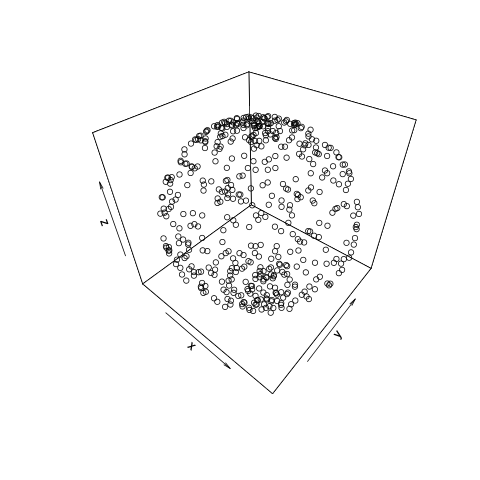
\includegraphics[width=\linewidth]{/home/andrew/Documents/Capstone/results/spherePoints.png}
  \caption{Scatterplot of 500 points in $S^2$.}
  \label{fig:sub1}
\end{subfigure}%
\begin{subfigure}{.5\textwidth}
  \centering
  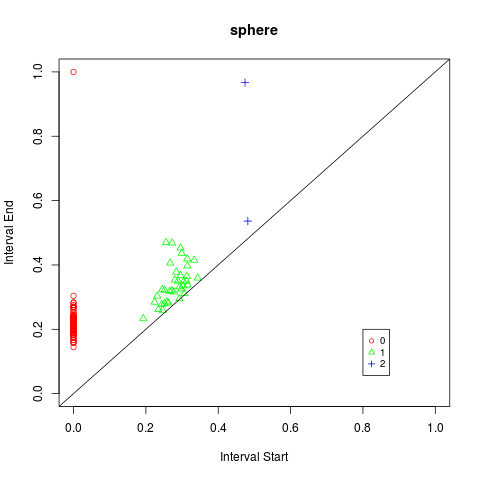
\includegraphics[width=\linewidth]{/home/andrew/Documents/Capstone/results/sphere_PersistanceDiagram.png}
  \caption{Persistence diagram for the set of points.}
  \label{fig:sub2}
\end{subfigure}
\caption{The persistent homology of randomly selected points from the sphere.}
\label{fig:test}
\end{figure}


Now we are ready to examine the topology of the countries of the world. The point cloud is simply the set of centroids in cartesian coordinates. The strong 2-hole disappears since countries do not wrap around the globe evenly. Circles appear relatively lately, so one possibility is that they form the boundary of large bodies of water where the countries link up around - perhaps with island nations acting as a bridge across the southern part of the body. Unfortunatley, \emph{phom}, our software of choice,  does not permit the study of the simplicial complexes directly, so another approach is needed to descern which countries generate these circles. 

\begin{figure}
\centering
\begin{subfigure}{.5\textwidth}
  \centering
  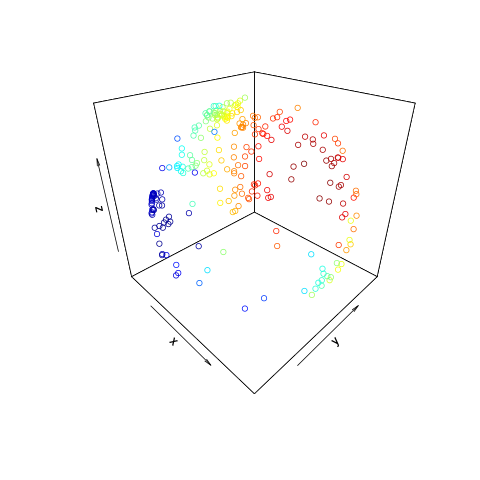
\includegraphics[width=\linewidth]{/home/andrew/Documents/Capstone/results/geoPoints.png}
  \caption{Scatterplot of Country centroids, a subset of $S^2$.  Centroids colored by lattitude, oriented with the north pole in the usual position.}
  \label{fig:sub1}
\end{subfigure}%
\begin{subfigure}{.5\textwidth}
  \centering
  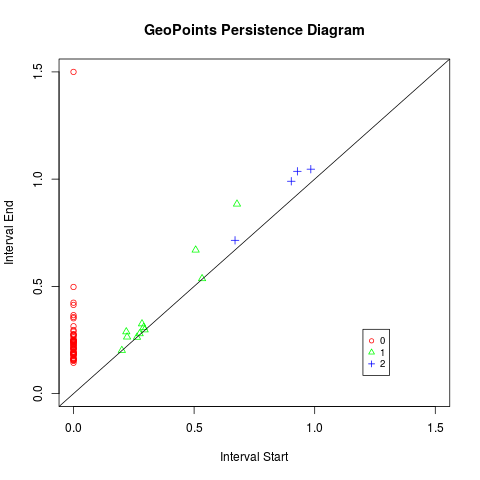
\includegraphics[width=\linewidth]{/home/andrew/Documents/Capstone/results/GeopointsPersistence}
  \caption{Persistence diagram for country centroids.}
  \label{fig:sub2}
\end{subfigure}
\caption{The persistence homology of country geography.}
\label{fig:geography}
\end{figure}

\section{TDA: Social Geography}

Taking the persistent homology of country geography as a baseline, we then add social indicators as extra dimensions and observe the effects on the persistent homology. First, we  require some notion of distnance in these social dimensions. To remedy the problem of noncommutative dimensions, we scale the data onto the interval $[-1,1]$, where an advantageous value is closer to positive one, and a disadvantageous value is closer to negative one. In this way, a country with disadvantageous results will be closer in distance with other countries with disadvantageous results, and the same is true with positive results. 

Thus  distinct clusters, partitions, or connected-components (however we choose to describe such groupings) indicate a finer division of countries based on measurable indicators of quality. Combining this information with geographic data then sheds light on whether regions of countries reflect these divisions. 

With addition of the indicators \emph{Income Per Person} and \emph{Life Expectancy}, an additional connected component arises in the form of a non-trivial $b_0 = 2 $ over the parameter range $[0,0.96]$. We see that all topological features washes out at about $\epsilon = 1.2$. The aforementioned second connected component may be considered significant since it persists over most of this range. Hence we observe initial evidence of a division of countries on geographic, health, and economic lines that did not exist before with just the geographic data. To understand this division, and discern how much water it holds, we examine the data by finding clusters with $k$-means, a standard clustering algorithm.

\begin{figure}
\centering
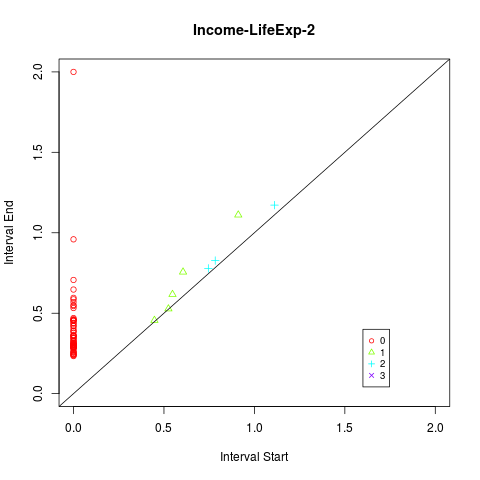
\includegraphics[width=.6\linewidth]{/home/andrew/Documents/Capstone/results/Income-LifeExp-2_PersistanceDiagram.png}
\caption{Persistance diagram of the data in five dimensions: geographic location, income per person, and life expectancy. Note the 0-hole that persists out to time 0.96, indicating a nontrival second connected component.}
\label{fig:geography}
\end{figure}


\section{Finding Clusters of Countries}

The $k$-means algorithm depends on a a method for dividing a set of points into regions known as  Voronoi regions. This partitioning scheme is known as the Voronoi Diagram.

\begin{defn} \cite{voronoi}
  A \emph{Voronoi Diagram} is a partitioning of a plane with n points into convex polygons such that each polygon contains exactly one generating point and every point in a given polygon is closer to its generating point than to any other. 
\end{defn}

The Voronoi Diagram can be generalized to higher dimensions, but it requires making the boundary of the regions fuzzy in order to be computationally feasable.  

\begin{defn}
  \emph{$k$-means clustering} is a method for partitioning a data set into $k$ clusters by the following algorithm:
  \begin{enumerate}
  \item A set of $k$ points $\set{\alpha_i}_0^k$ are assigned (often randomly) to represent the cluster centers.
  \item The Voronoi diagram partitions the data into sets $\set{A_i}_0^k$ about the cluster centers $\set{\alpha_i}_0^k$.
  \item Cluster centers are reassigned to the arithmetic mean of the points within the particular region, e.g. for some set $A_i$ centered at $\alpha_i$: 
\[ \alpha_i' = \frac{1}{|A_i|}\sum_{x_j \in A_i} x_j \]
  \item Steps (2)-(3) are repeated until the cluster centers converge. 
  \end{enumerate}

\end{defn}

\begin{figure}
  \centering
  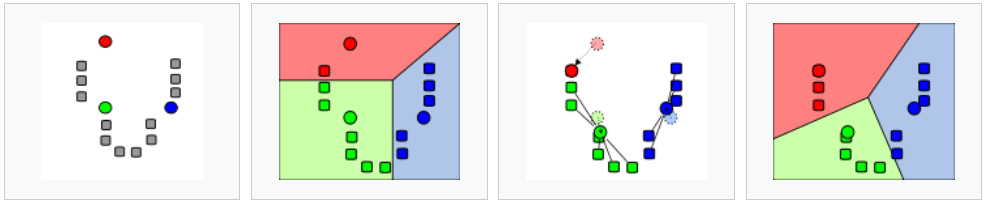
\includegraphics[width=\linewidth]{kmeans.png}
  \caption{Diagram of $k$-means alogrithm. \cite{wikimedia}}
  \label{fig:kmeans}
\end{figure}

As with the initial persistent homology analysis, we first look at clusters based soley on geographic proximity. One drawback of the $k$-means is that it requires a predetermined choice of $k$, the number of clusters. The \emph{pamk} function (R, \emph{fpc} package) implements an algorithm that makes an intelligent guess at the number of clusters by comparing the results of multpile values of $k$. For soley geographic data, \emph{pamk} finds seven distinct clusters that basically coincide with the continents. However, the regions collapse into four when data on Life Expectancy and Income per Person is incluced. Interstingly, but perhaps not surprisingly, northern and southern Africa are pulled toegether and made more distinct from European countries. On the other hand, Asian and countries of the South Pacific are brought together. 



\begin{figure}
\centering
\begin{subfigure}{.5\textwidth}
  \centering
  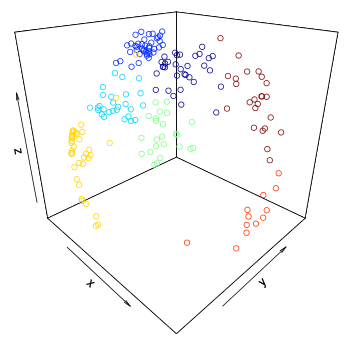
\includegraphics[width=\linewidth]{/home/andrew/Documents/Capstone/results/geo_Clusters(2).png}
  \caption{$k$ = 7. Clusters based on geographic data only.}
  \label{fig:sub1}
\end{subfigure}%
\begin{subfigure}{.5\textwidth}
  \centering
  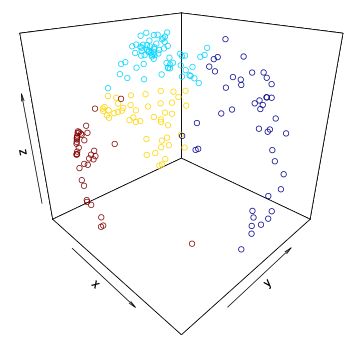
\includegraphics[width=\linewidth]{/home/andrew/Documents/Capstone/results/inc-lifeExp-geo_Clusters(2).png}
  \caption{$k$ = 4. Combined Geographic, Life expectancy, and Income per person data. See Appendix A for a list of countries by region.}
  \label{fig:sub2}
\end{subfigure}
\caption{Results of clustering by geographic data and the addition of social data.}
\label{fig:culster}
\end{figure}


\section{Discussion and further work}

We have a natural tendancy to group countries in certain regions together not solely on geography but also on perceived social/polital trends. The results of preliminary TDA and clustering analysis show that this tendancy partly reflects reality. Further work is surely needed to see how far these distinctions run in the data, after all we have examined only two out of the hundreds of indicators available on the Gapminder site alone. While it is too early to make strong claims about the division of countries, it is notable how life expactancy and income per person - two indicators that represent the collusion of a wide swath of economic and health phenomena - seem to pull countries into certain geographic regions. 

Why TDA? It may seem that these results could have been derived soley from an analysis of data clusters. The comparison itself is interesting. Can zero-order persistent homology serve as a clustering algorithm in its own right? Certain precautions must be taken. For example, the number of connect components of a simplicial complex based on point cloud data is highly sensitive to outliers - if a point lives very far away from its neighbors, then it will take a large filtration time to eliminate its undesireable contribution to $b_0$. 

Careful consideration must also be taken with how long a component should persist before considering it significant. For example, a data set may have a baseline density such that what we would consider distinct components are joined up prematurely. Sensitive to density in that it cannot distinguish features of uniform density unless they are spaced sufficiently far apart.

Despite these drawbacks, persistent homology does have some advantages. Unlike k-means, it does not require a predetermined choice in the number of clusters to look for. Also by restriciting yourself to particular ranges in filtration time you can examine clusters at desired densities, hopefully with the benefit of distinguishing fine from coarse structure. At the least, homology could put bounds on the ideal number of clusters to inform the use of algorithms such as k-means. This topic deserves more attention, since as TDA rises in usage it is only to our benefit to understand all possible uses of the data it gives.

%Would like to include an appendix about all the sweet R-code that I wrote, but maybe it's not too imporant / worth my time right now. 
%\newpage 
%\section*{Appendix A: Preparing the data}
%...Actually PAM uses k-medoid which chooses data points as the centers and minimizes the pairwise distance between points. Still very similar. 

\newpage
\section*{Appendix A: Countries by Region}

\begin{figure}[b]
\centering
\tiny\begin{tabular}{|l|l|l|l|}
\hline
Region 1 (Dark Blue) & Region 2 (Light Blue) &Region 3 (Yellow) &Region 4 (Red)\\
\hline
Afghanistan&Albania&Angola&Antigua and Barbuda \\
Australia&Algeria&Benin&Argentina \\
Bangladesh&Armenia&Botswana&Aruba \\
Bhutan&Austria&Burkina Faso&Bahamas\\
Brunei&Azerbaijan&Burundi&Barbados\\
Cambodia&Bahrain&Cameroon&Belize\\
China&Belarus&Central African Rep.&Bolivia\\
Fiji&Belgium&Chad&Brazil\\
Guam&Bosnia and Herzegovina&Comoros&Cape Verde\\
Hong Kong, China&Bulgaria&Congo, Dem. Rep.&Chile\\
India&Canada&Congo, Rep.&Colombia\\
Indonesia&Croatia&Cote d'Ivoire&Costa Rica\\
Japan&Cyprus&Djibouti&Cuba\\
Kiribati&Czech Rep.&Equatorial Guinea&Dominican Rep.\\
Korea, Dem. Rep.&Denmark&Eritrea&Ecuador\\
Korea, Rep.&Egypt&Ethiopia&El Salvador\\
Kyrgyzstan&Estonia&Gabon&French Guiana\\
Laos&Finland&Gambia&French Polynesia\\
Macao, China&France&Ghana&Grenada\\
Malaysia&Georgia&Guinea&Guadeloupe\\
Maldives&Germany&Guinea-Bissau&Guatemala\\
Mauritius&Greece&Kenya&Guyana\\
Mayotte&Greenland&Lesotho&Haiti\\
Mongolia&Hungary&Liberia&Honduras\\
Nepal&Iceland&Madagascar&Jamaica\\
New Caledonia&Iran&Malawi&Martinique\\
New Zealand&Iraq&Mali&Mexico\\
Pakistan&Ireland&Mauritania&Nicaragua\\
Papua New Guinea&Israel&Mozambique&Panama\\
Philippines&Italy&Namibia&Paraguay\\
Reunion&Jordan&Niger&Peru\\
Russia&Kazakhstan&Nigeria&Puerto Rico\\
Samoa&Kuwait&Rwanda&Saint Lucia\\
Seychelles&Latvia&Sao Tome and Principe&Saint Vincent and the Grenadines\\
Singapore&Lebanon&Senegal&Suriname\\
Solomon Islands&Libya&Sierra Leone&Trinidad and Tobago\\
Sri Lanka&Lithuania&Somalia&United States\\
Taiwan&Luxembourg&South Africa&Uruguay\\
Tajikistan&Macedonia, FYR&South Sudan&Venezuela\\
Thailand&Malta&Sudan&\\
Timor-Leste&Moldova&Swaziland&\\
Tokelau&Montenegro&Tanzania&\\
Tonga&Morocco&Togo&\\
Vanuatu&Netherlands&Uganda&\\
Vietnam&Norway&Yemen, Rep.&\\
&Oman&Zambia&\\
&Poland&Zimbabwe&\\
&Portugal&&\\
&Qatar&&\\
&Romania&&\\
&Saudi Arabia&&\\
&Serbia&&\\
&Slovak Republic&&\\
&Slovenia&&\\
&Spain&&\\
&Sweden&&\\
&Switzerland&&\\
&Syria&&\\
&Tunisia&&\\
&Turkey&&\\
&Turkmenistan&&\\
&Ukraine&&\\
&United Arab Emirates&&\\
&United Kingdom&&\\
&Uzbekistan&&\\
&West Bank and Gaza&&\\
&Western Sahara&&\\
\hline
\end{tabular}
\caption{Result of clustering based on geographic data, income per person, and life expectancy. This table corresponds to plot (b) of Figure 5.}
\end{figure} 

\newpage
\begin{thebibliography}{11}

\bibitem{gapminder}
 Gapminder website, data files. 
"Gapminder: Unveiling the Beauty of Statistics for a Fact Based World View." Gapminder. N.p., n.d. Web. 13 Dec. 2014.

\bibitem{Crossley}
 Crossley, Martin D. \emph{Essential Topology}. London: Springer, 2005. Print. 

\bibitem{carlsson}
 Gunnar Carlsson, “Topology and Data,” \emph{Bulletin of the American Mathematical Society} 46, no. 2 (2009): 255–308.

\bibitem{ghrist}
 Robert Ghrist, “Barcodes: The Persistent Topology of Data,” \emph{Bulletin of the American Mathematical Society} 45, no. 1 (2008): 61.

\bibitem{comptop}
Edelsbrunner, Herbert, and J. Harer. \emph{Computational Topology: An Introduction}. Providence, RI: American Mathematical Society, 2010. Print. 

\bibitem{wikimedia}
"K Means Example Step 1." - Wikimedia Commons. N.p., n.d. Web. 13 Dec. 2014.

\bibitem{voronoi}
"Voronoi Diagram." Wolfram MathWorld. N.p., n.d. Web. 13 Dec. 2014.

\end{thebibliography}
\end{document}


